\documentclass[aspectratio=169,11pt]{beamer}

\usetheme{metropolis}
\setbeamertemplate{caption}{\raggedright\insertcaption\par}
\setbeamertemplate{frame numbering}[fraction]

\usepackage[utf8]{inputenc}
\usepackage{amsmath,amssymb}
\usepackage{booktabs}
\usepackage{tabularx}
\usepackage{tikz}
\usepackage{graphicx}
\usepackage{hyperref}
\usepackage{bbm}

\usetikzlibrary{arrows,positioning,shapes}

\title{Zero-shot Transfer of Single-Crane DRL Policies \\ for Multi-Crane Container Retrieval}
\author{PhD Candidate --- AI/ML/DL/Optimization}
\date{}

\begin{document}

\maketitle

\begin{frame}{Problem: Container Retrieval Problem}
\begin{columns}
\begin{column}{0.55\textwidth}
\textbf{CRP:} NP-hard optimization in container terminals
\begin{itemize}
    \item Yard: $B$ bays $\times$ $R$ rows $\times$ $T$ tiers
    \item $N$ containers với retrieval priority $\{1,\dots,N\}$
    \item Cần relocate blocking containers để retrieve
    \item \textbf{Mục tiêu:} Minimize total working time
\end{itemize}

\vspace{0.5cm}
\textbf{Giới hạn của SOTA:}
\begin{itemize}
    \item Shin et al. (2026, TR-C): DRL cho \textbf{single-crane}
    \item 7.8\% gap vs lower bound trên Lee benchmark
\end{itemize}
\end{column}
\begin{column}{0.45\textwidth}
\centering
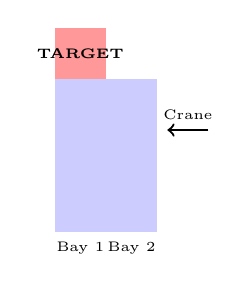
\begin{tikzpicture}[scale=0.65]
\fill[blue!20] (0,0) rectangle (1,1);
\fill[blue!20] (0,1) rectangle (1,2);
\fill[blue!20] (0,2) rectangle (1,3);
\fill[red!40]  (0,3) rectangle (1,4);
\fill[blue!20] (1,0) rectangle (2,1);
\fill[blue!20] (1,1) rectangle (2,2);
\fill[blue!20] (1,2) rectangle (2,3);
\node at (0.5,3.5) {\tiny\textbf{TARGET}};
\node at (0.5,-0.3) {\tiny Bay 1};
\node at (1.5,-0.3) {\tiny Bay 2};
\draw[->,thick] (3,2) -- (2.2,2) node[midway,above] {\tiny Crane};
\end{tikzpicture}
\end{column}
\end{columns}
\end{frame}

\begin{frame}{Research Gap}
\begin{block}{Thực tế}
Real-world terminal vận hành \textbf{2--3 cranes} trên cùng yard block để đáp ứng throughput.
\end{block}

\begin{block}{Khoảng trống}
\begin{itemize}
    \item Toàn bộ CRP research (15+ năm): chỉ single-crane
    \item M-CRP chưa được định nghĩa
    \item Chưa có lower bound, benchmark, method cho multi-crane
    \item Không biết single-crane policy có zero-shot transfer được không
\end{itemize}
\end{block}

\vspace{0.3cm}
\centering\textbf{\large Research Question:}
\vspace{0.2cm}
\par\centering\emph{\textquote{Can a single-crane DRL policy be transferred zero-shot to multi-crane environments?}}
\end{frame}

\begin{frame}{Contributions (5 Claims)}
\begin{enumerate}
    \item[{[C1]}] \textbf{Formal M-CRP definition} + NP-hardness proof
    \item[{[C2]}] \textbf{M-CRP Lower Bound (Theorem~3)} — $\LB_{\text{MCRP}}$ \\ 
        $\LB_{\text{MCRP}} = \LB_{\text{retrieval}} + \frac{\LB_{\text{relocation}}}{C} + \LB_{\text{interference}}$
    \item[{[C3]}] \textbf{4 Crane Assignment Strategies} cho zero-shot transfer
    \item[{[C4]}] \textbf{First empirical evaluation}: 140 instances, 1,120 runs
    \item[{[C5]}] \textbf{Public benchmark dataset} (CC BY 4.0)
\end{enumerate}
\end{frame}

\begin{frame}{Method: Decoupled Inference Architecture}
\begin{center}
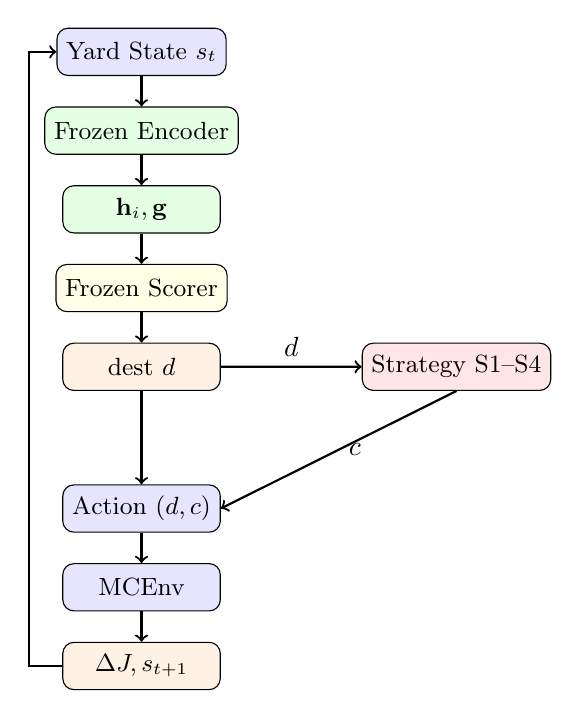
\begin{tikzpicture}[node distance=1cm, auto, scale=0.85]
\tikzstyle{block} = [rectangle, draw, rounded corners, minimum width=2cm, minimum height=0.6cm, text centered, font=\small]
\tikzstyle{arrow} = [->, thick]

\node (state) [block, fill=blue!10] {Yard State $s_t$};
\node (enc) [block, below of=state, fill=green!10] {Frozen Encoder};
\node (emb) [block, below of=enc, fill=green!10] {$\mathbf{h}_i, \mathbf{g}$};
\node (score) [block, below of=emb, fill=yellow!10] {Frozen Scorer};
\node (dest) [block, below of=score, fill=orange!10] {dest $d$};
\node (strat) [block, right of=dest, xshift=3cm, fill=red!10] {Strategy S1--S4};
\node (action) [block, below of=dest, yshift=-0.8cm, fill=blue!10] {Action $(d,c)$};
\node (env) [block, below of=action, fill=blue!10] {MCEnv};
\node (cost) [block, below of=env, fill=orange!10] {$\Delta J, s_{t+1}$};
\draw[arrow] (state)--(enc); \draw[arrow] (enc)--(emb);
\draw[arrow] (emb)--(score); \draw[arrow] (score)--(dest);
\draw[arrow] (dest)--(action);
\draw[arrow] (dest.east)--node[above]{$d$}(strat.west);
\draw[arrow] (strat.south)--node[right]{$c$}(action.east);
\draw[arrow] (action)--(env); \draw[arrow] (env)--(cost);
\draw[arrow] (cost.west)--++(-0.5,0)|-(state.west);
\end{tikzpicture}
\end{center}
\end{frame}

\begin{frame}{4 Crane Assignment Strategies}
\begin{table}[h]
\centering
\begin{tabular}{lcc}
\toprule
Strategy & Mechanism & Complexity \\
\midrule
\textbf{S1 RoundRobin} & Cyclic task assignment & $O(1)$ \\
\textbf{S2 ZoneSplit} & Static bay zones per crane & $O(B)$ \\
\textbf{S3 LoadBalance} & Min-count task assignment & $O(C)$ \\
\textbf{S4 GreedyOptimal} & 1-step lookahead cost min & $O(C^2)$ \\
\bottomrule
\end{tabular}
\end{table}

\vspace{0.3cm}
\textbf{Key design:}
\begin{itemize}
    \item S1, S3: \textbf{spatially unaware} (baselines)
    \item S2, S4: \textbf{spatially aware} (leverage crane position)
\end{itemize}
\end{frame}

\begin{frame}{Experimental Setup}
\begin{columns}
\begin{column}{0.5\textwidth}
\textbf{Dataset:}
\begin{itemize}
    \item 140 M-CRP instances từ Lee benchmark
    \item 2-3 cranes, 2 yard scales
    \item Random + upside-down distributions
\end{itemize}
\end{column}
\begin{column}{0.5\textwidth}
\textbf{Config:}
\begin{itemize}
    \item Model: Shin et al. epoch(100) — public
    \item 0 GPU (CPU laptop only)
    \item 1,120 total runs ($\approx$60 phút)
    \item Backward compatibility verified: $<2\%$ diff
\end{itemize}
\end{column}
\end{columns}
\end{frame}

\begin{frame}{Single-Crane Results}
\begin{center}
\begin{tabular}{lcccc}
\toprule
Method & Mean Gap(\%) & Min(\%) & Max(\%) \\
\midrule
Random & 68.72 & 47.16 & 104.26 \\
Kim2016 & 25.02 & 13.27 & 37.52 \\
Lin2015 & 10.28 & 5.55 & 14.14 \\
\midrule
\textbf{ZeroShot (ours)} & \textbf{5.63} & \textbf{4.27} & \textbf{7.04} \\
\bottomrule
\end{tabular}
\end{center}

\vspace{0.3cm}
\centering\textbf{ZeroShot outperforms Lin2015 (SOTA heuristic) by 4.65pp!}
\end{frame}

\begin{frame}{Multi-Crane Results}
\begin{table}[h]
\centering
\begin{tabular}{lcccc}
\toprule
Strategy & C=2 gap(\%) & C=3 gap(\%) & Intf(C=2) & Intf(C=3) \\
\midrule
S1 RoundRobin & 10.99 & 11.19 & 105.9 & 147.2 \\
\textbf{S2 ZoneSplit} & \textbf{10.46} & \textbf{10.71} & \textbf{0.5} & \textbf{0.7} \\
S3 LoadBalance & 10.99 & 11.19 & 105.9 & 147.2 \\
S4 GreedyOptimal & 10.48 & 10.75 & 0.0 & 0.0 \\
\bottomrule
\end{tabular}
\end{table}

\vspace{0.3cm}
\textbf{Key findings:}
\begin{itemize}
    \item S2 ZoneSplit: \textbf{best gap} + \textbf{$\sim$0 interference} + \textbf{$O(B)$ complexity}
    \item S2 vs S4: không significant difference ($p > 0.1$)
    \item Spatial awareness $>$ task balancing
\end{itemize}
\end{frame}

\begin{frame}{Results by Yard Scale}
\begin{columns}
\begin{column}{0.55\textwidth}
\begin{table}[h]
\centering
\begin{tabular}{lccc}
\toprule
Scale & S1(\%) & S2(\%) & S4(\%) \\
\midrule
\multicolumn{4}{l}{\textbf{C=2}} \\
Small (1-4 bays) & 9.26 & 9.04 & 9.02 \\
Medium (6-10 bays) & 13.60 & \textbf{12.58} & 12.68 \\
\midrule
\multicolumn{4}{l}{\textbf{C=3}} \\
Small (1-4 bays) & 8.43 & 8.24 & 8.34 \\
Medium (6-10 bays) & 15.33 & \textbf{14.41} & 14.36 \\
\bottomrule
\end{tabular}
\end{table}
\end{column}
\begin{column}{0.45\textwidth}
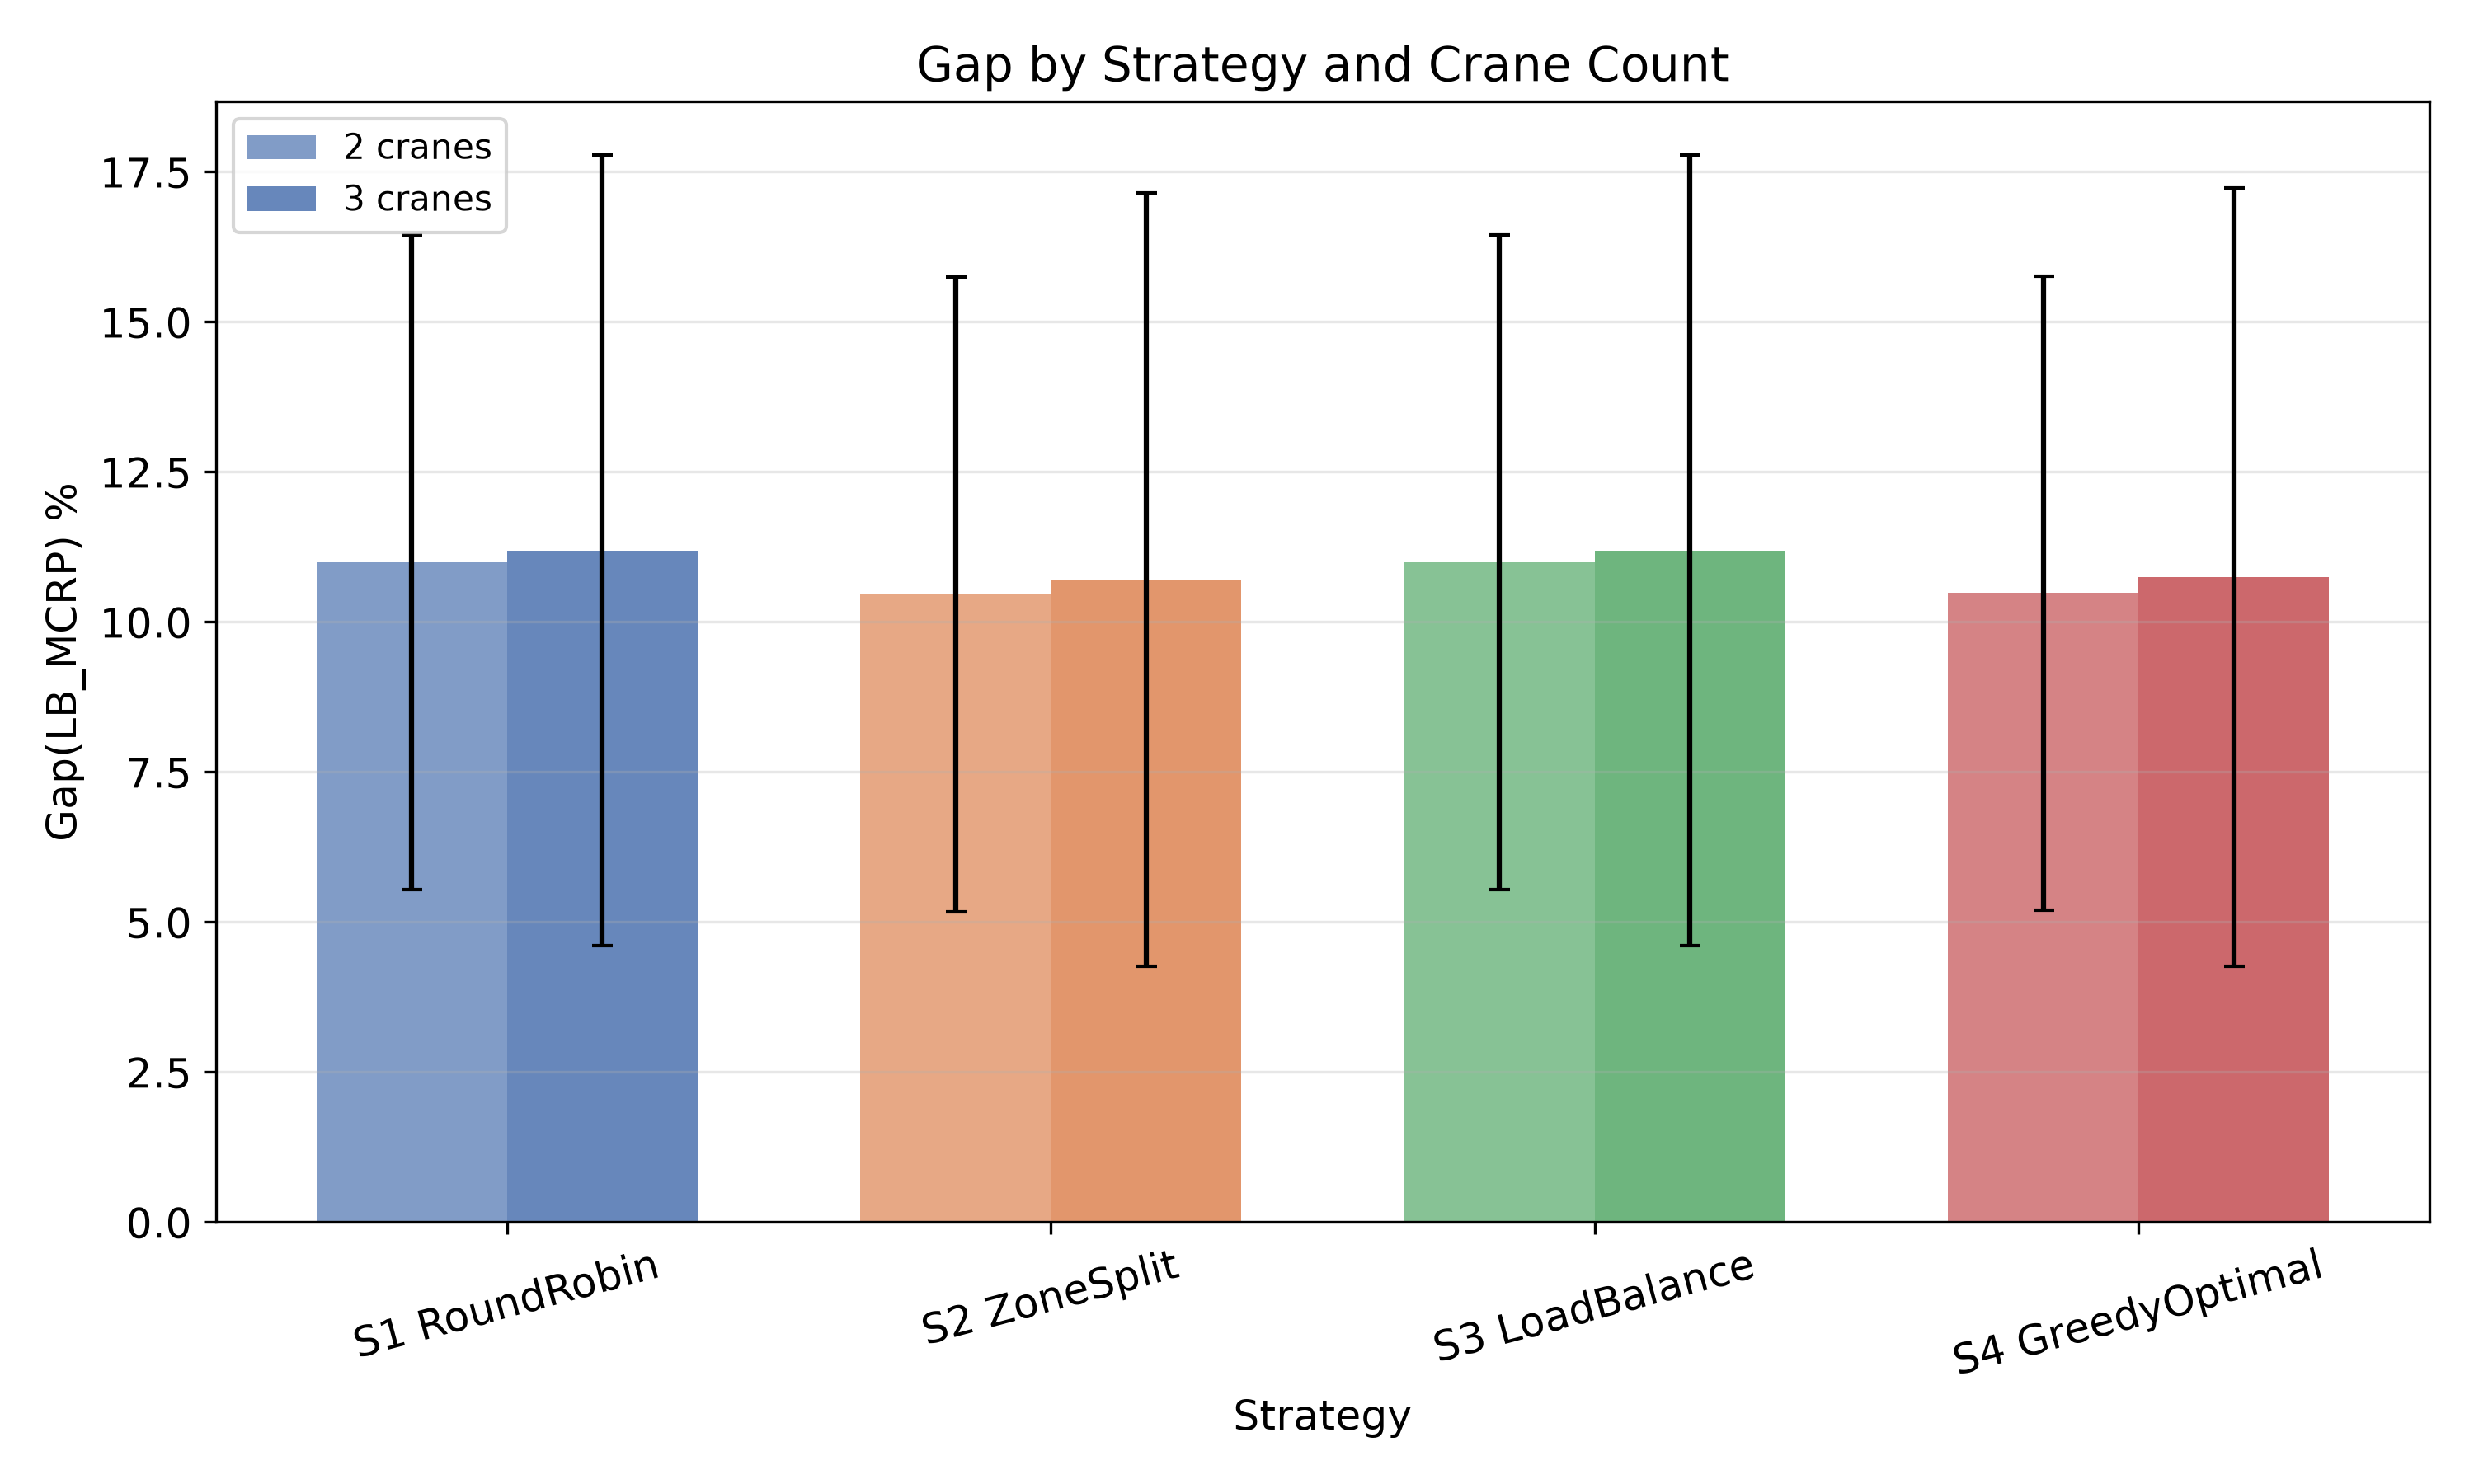
\includegraphics[width=\textwidth]{../../results/figures/fig1_gap_by_strategy.png}
\end{column}
\end{columns}
\vspace{0.2cm}
\centering\textbf{Spatial strategies improve as yard scale grows}
\end{frame}

\begin{frame}{Statistical Significance}
\begin{table}[h]
\centering
\begin{tabular}{lccc}
\toprule
Pair & C=2 $p$ & C=3 $p$ & Significant? \\
\midrule
S2 vs S1 & $<0.001$ & $<0.001$ & Yes \\
S4 vs S1 & $<0.001$ & $<0.001$ & Yes \\
S2 vs S4 & 0.128 & 0.534 & No \\
\bottomrule
\end{tabular}
\end{table}

\vspace{0.3cm}
\begin{itemize}
    \item \textbf{S2, S4 significantly outperform S1, S3} (Wilcoxon, $p < 0.001$)
    \item S2 vs S4: \textbf{no significant difference} $\Rightarrow$ simple ZoneSplit is sufficient
\end{itemize}
\end{frame}

\begin{frame}{Interference Analysis}
\begin{columns}
\begin{column}{0.5\textwidth}
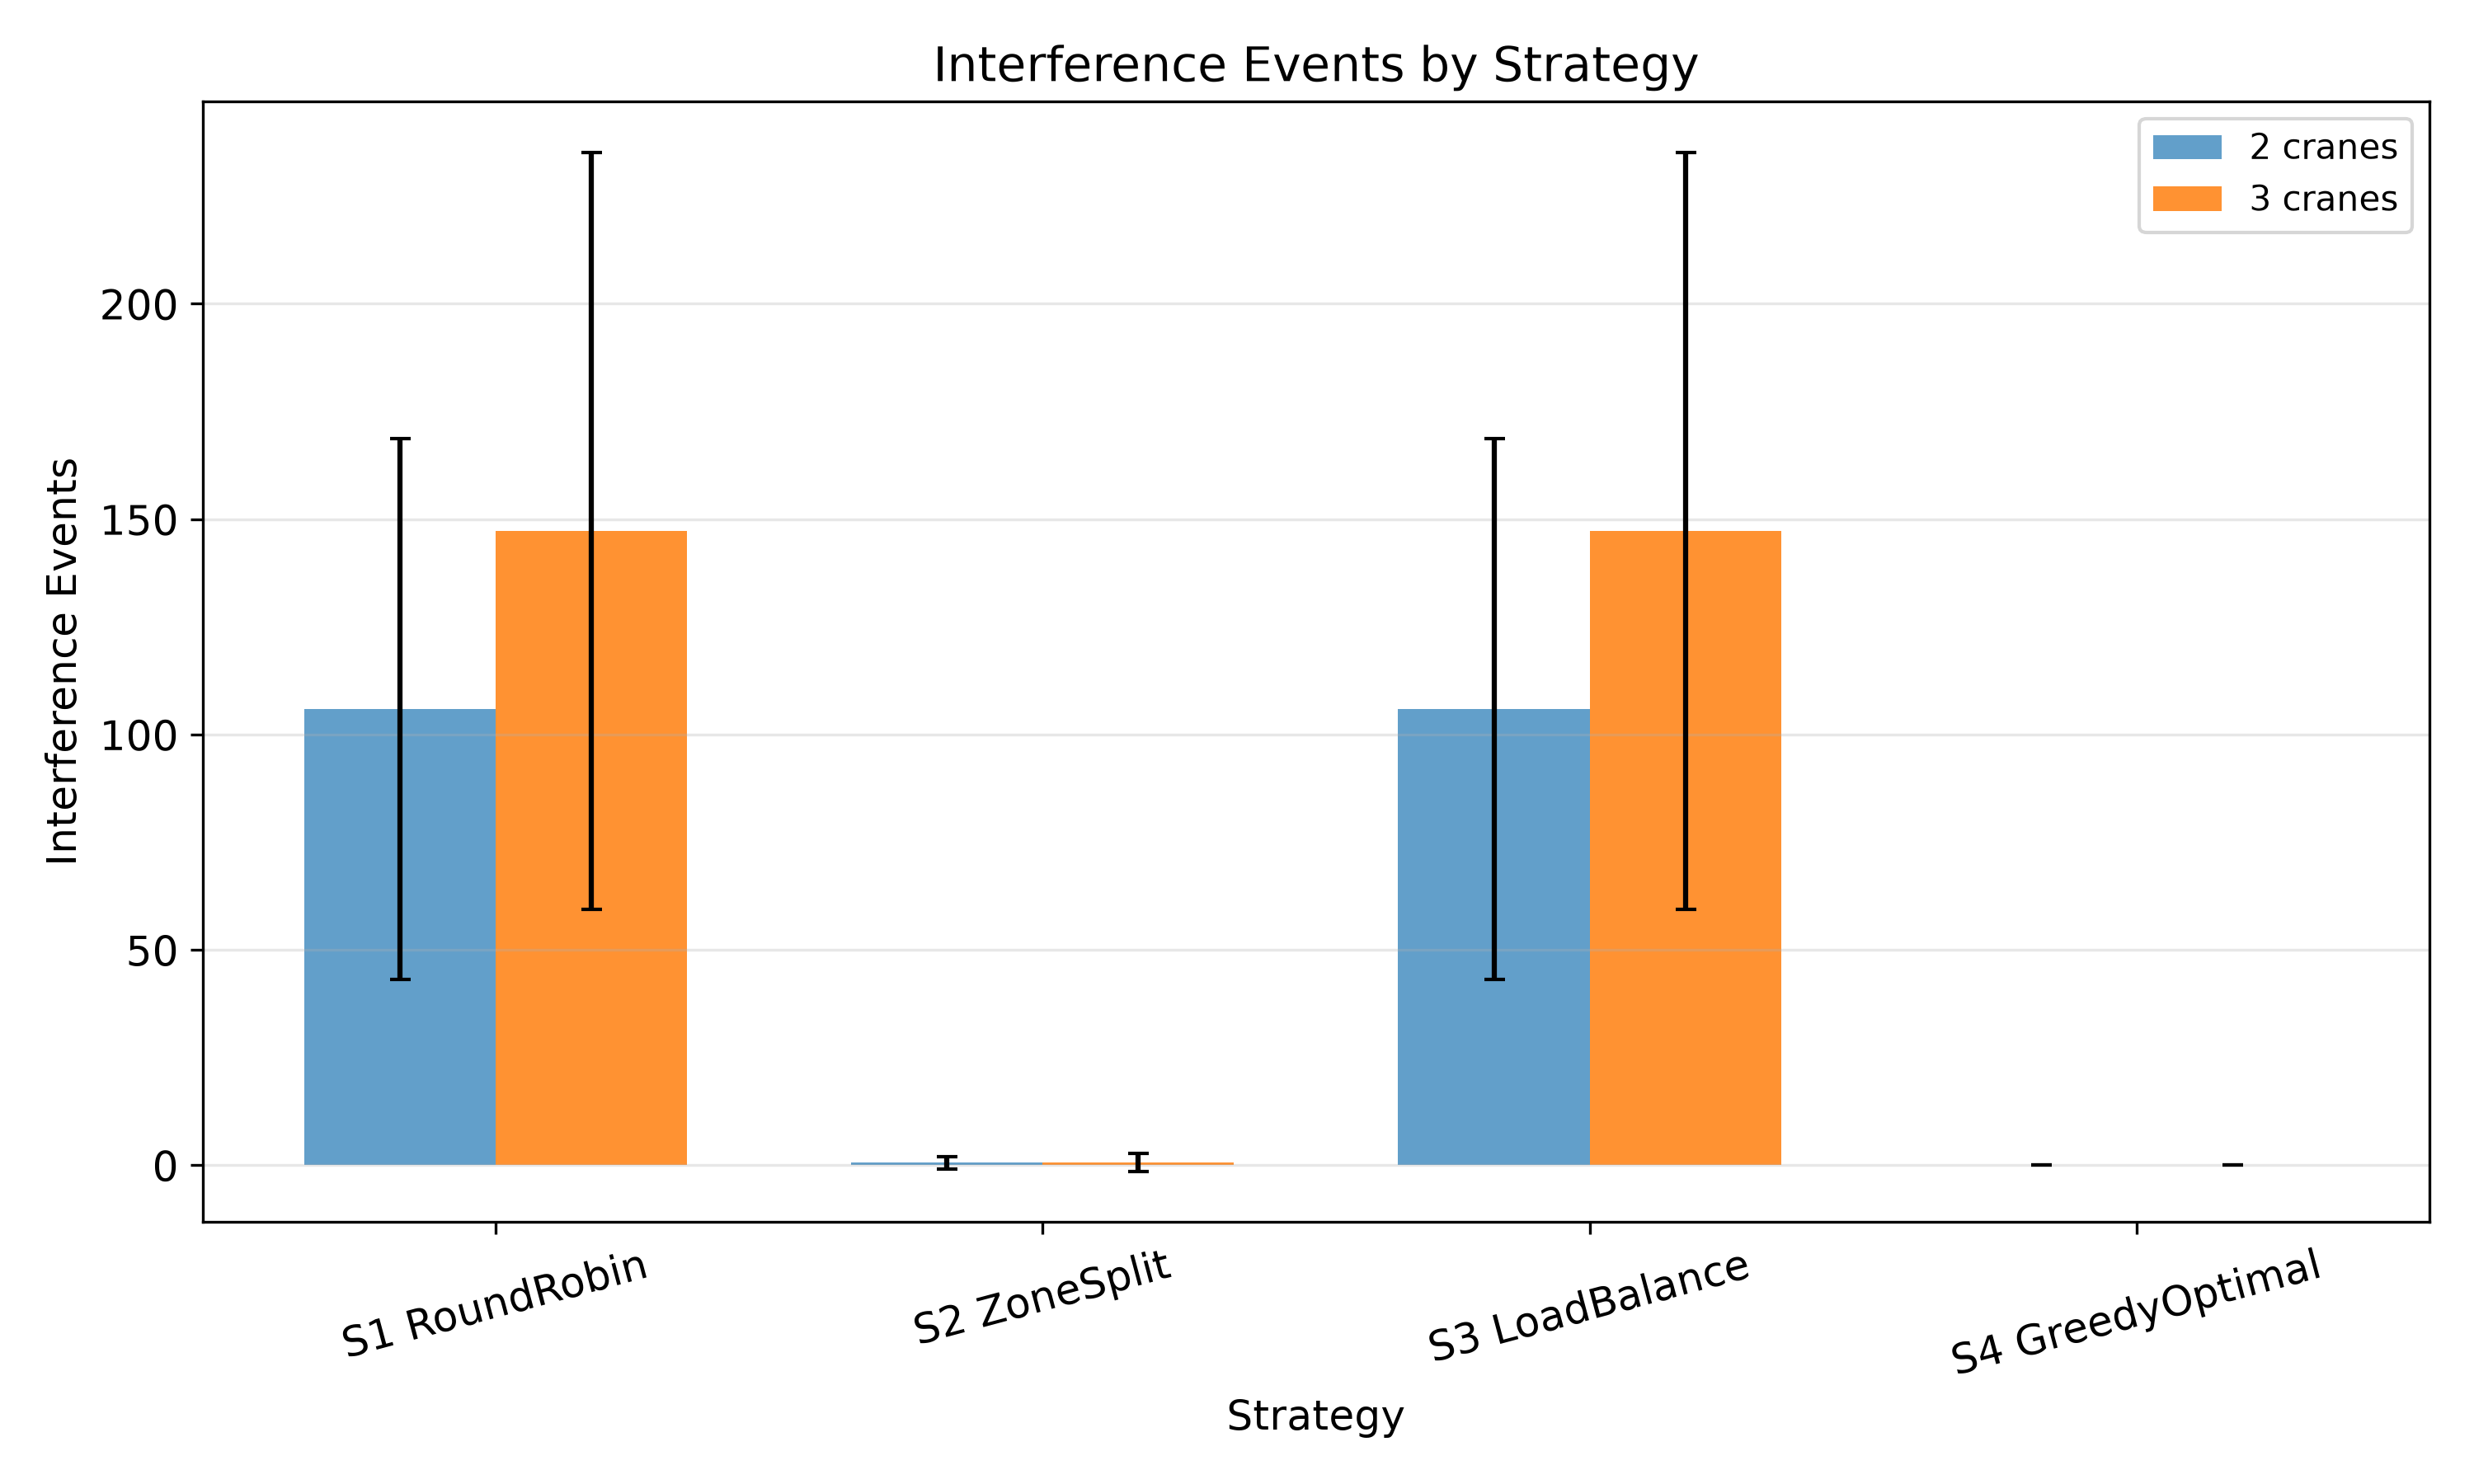
\includegraphics[width=\textwidth]{../../results/figures/fig4_interference.png}
\end{column}
\begin{column}{0.5\textwidth}
\textbf{Interference reduction:}
\begin{itemize}
    \item S1: 105.9 events (C=2)
    \item S3: 105.9 events
    \item \textbf{S2: 0.5 events ($>$99.5\% reduction)}
    \item S4: 0.0 events
\end{itemize}
\vspace{0.3cm}
Spatial awareness eliminates interference without complex coordination!
\end{column}
\end{columns}
\end{frame}

\begin{frame}{Why ZoneSplit Works}
\begin{block}{Key insight}
Single-crane DRL policy học cách relocate containers đến stacks gần đó. ZoneSplit align với behavior này: mỗi crane operate trong zone riêng.
\end{block}

\vspace{0.3cm}
\textbf{Practical recommendations:}
\begin{itemize}
    \item \textbf{ZoneSplit (S2)} recommend cho deployment
    \item 0 GPU training cost
    \item $O(B)$ complexity per decision
    \item Align với existing terminal zoning practices
\end{itemize}
\end{frame}

\begin{frame}{Limitations}
\begin{enumerate}
    \item \textbf{Sequential simulation} — serializes crane actions
    \begin{itemize}
        \item Speedup C2$\to$C3: only 1.01$\times$ (parallel model: $\approx$1.5$\times$)
        \item Affects all strategies equally — no bias
    \end{itemize}
    \item \textbf{LB looseness} at $C>1$ — negative gaps observed
    \item \textbf{Single-crane verification} — subset of full benchmark
\end{enumerate}

\vspace{0.3cm}
\textbf{Future work:}
\begin{itemize}
    \item Fine-tuning policy on multi-crane data
    \item Multi-agent RL from scratch
    \item Parallel simulation model
\end{itemize}
\end{frame}

\begin{frame}{Conclusion}
\begin{enumerate}
    \item \textbf{Zero-shot transfer \underline{works}} — 10.5\% gap without retraining
    \item \textbf{ZoneSplit best} — lowest gap, 0 interference, $O(B)$
    \item \textbf{Spatial awareness $>$ task balancing} 
    \item \textbf{First M-CRP study} — definition, bound, benchmark
\end{enumerate}

\vspace{0.5cm}
\centering
\fbox{\parbox{0.8\textwidth}{\centering Code + Dataset + Paper:\\
\url{https://github.com/sutobode/Master}}}
\end{frame}

\begin{frame}{Q\&A}
\centering
\vspace{1cm}
{\Huge Thank You!}
\vspace{0.5cm}

\Large Questions?
\end{frame}

\end{document}
